\documentclass[pdflatex,sn-mathphys-num]{sn-jnl}

\usepackage{graphicx}
\usepackage{booktabs}
\usepackage{subcaption}
\usepackage{amsmath,amssymb}
\usepackage{hyperref}

\raggedbottom

\begin{document}

\title[EDA para Predicción de Riesgo Crediticio]{Análisis Exploratorio de Datos para la Predicción de Riesgo Crediticio: el caso \textit{Give Me Some Credit}}

\author*[1]{\fnm{Valeria} \sur{Flórez}}\email{florezvaleria@uninorte.edu.co}

\author[1]{\fnm{Katherin} \sur{Barrera}}\email{lkatherin@uninorte.edu.co}

\affil*[1]{\orgdiv{Departamento de Matemáticas, Física y Ciencia de Datos}, \orgname{Universidad del Norte}, \orgaddress{\city{Barranquilla}, \country{Colombia}}}

\abstract{Este documento presenta la primera fase de un proyecto de clasificación de riesgo crediticio, desarrollado sobre el conjunto de datos público \textit{Give Me Some Credit} (Kaggle), compuesto por 150{,}000 instancias y 11 variables financieras y de comportamiento de los clientes. En esta etapa se realiza el proceso de \textit{Extract-Transform-Load} (ETL) y un Análisis Exploratorio de Datos (EDA) exhaustivo, con el fin de comprender la estructura del conjunto de datos, identificar valores atípicos y faltantes, y sentar las bases para las decisiones de preprocesamiento y modelamiento. Tras la limpieza (imputación por mediana de dos variables con datos faltantes y eliminación de un registro con edad inválida), el dataset quedó con 149{,}999 filas sin valores nulos. El EDA reveló un fuerte desbalance de clases en la variable objetivo (93.32\% sin morosidad grave frente a 6.68\% con morosidad grave), asimetría positiva marcada en la mayoría de las variables numéricas, un código de valor especial (96/98) en las tres variables de conteo de atrasos que no representa un conteo real, y una anomalía en \texttt{DebtRatio} explicada por su cruce con los registros de ingreso no reportado. Dado el tamaño muestral (N $\approx$ 150{,}000), se evitaron pruebas formales de normalidad por exceso de potencia estadística, optando en su lugar por diagnósticos descriptivos de forma y por la prueba de Mann--Whitney U con tamaño de efecto corregido por empates (r de Rosenthal) y AUC univariado, aplicada uniformemente a ocho variables numéricas frente a la variable objetivo. El desarrollo del modelo predictivo, su evaluación y los resultados finales se abordarán y documentarán en las siguientes etapas del proyecto.}

\keywords{riesgo crediticio, clasificación binaria, análisis exploratorio de datos, valores atípicos, desbalance de clases}

\maketitle

\section{Introducción}\label{sec:intro}

El problema de predecir el riesgo de incumplimiento crediticio es central para las instituciones financieras, ya que una identificación temprana de clientes de alto riesgo permite mitigar pérdidas y ofrecer condiciones de crédito más justas. En este trabajo se aborda el conjunto de datos \textit{Give Me Some Credit}, publicado en Kaggle como parte de una competencia de \textit{credit scoring}~\cite{gmsc}, cuyo objetivo es estimar la probabilidad de que un cliente presente dificultades financieras graves en los siguientes dos años.

Trabajos recientes en \textit{credit scoring} han señalado que la calidad del análisis y del preprocesamiento de datos incide directamente en el desempeño de los modelos predictivos posteriores~\cite{ichim2025credit}, y que el fuerte desbalance de clases típico de estos conjuntos de datos requiere un tratamiento explícito, por ejemplo mediante técnicas de sobremuestreo como ADASYN~\cite{chia2025adasyn}. Estos hallazgos motivan a que, antes de entrenar cualquier modelo, se realice una comprensión profunda del conjunto de datos.

Este documento corresponde a la primera entrega del proyecto de aprendizaje automático y se concentra en las etapas previas al modelamiento: la comprensión del problema, el proceso de ETL y el Análisis Exploratorio de Datos (EDA). Estas etapas son fundamentales, ya que las decisiones de preprocesamiento que se tomen aquí (tratamiento de valores atípicos, del desbalance de clases y de códigos de valor especial) determinarán directamente la validez de los modelos que se entrenen posteriormente.

\section{Metodología}\label{sec:metodologia}

\subsection{Descripción del problema y del conjunto de datos}\label{subsec:datos}

Se utilizó el conjunto público \textit{Give Me Some Credit}, disponible en la plataforma Kaggle~\cite{gmsc}, correspondiente a una competencia de predicción de riesgo crediticio. El dataset original contiene 150{,}000 instancias y 11 variables, incluyendo información financiera y de comportamiento de los clientes (edad, ingresos mensuales, número de préstamos, utilización de líneas de crédito, historial de pagos y cantidad de veces que el cliente ha presentado retrasos en sus obligaciones financieras). La variable objetivo es \texttt{SeriousDlqin2yrs}, un indicador binario que señala si el cliente experimentó una situación de morosidad grave durante los dos años siguientes (1 = sí, 0 = no), lo que permite plantear el problema como una tarea de \textbf{clasificación binaria}. El conjunto presenta un fuerte desbalance de clases: 93.32\% de los clientes (139{,}973) no presentó morosidad grave, frente a solo 6.68\% (10{,}026) que sí la presentó.

\subsection{Proceso ETL}\label{subsec:etl}

\textbf{Extract.} Los datos crudos se descargaron desde la competencia oficial de Kaggle en formato \texttt{.csv} (\texttt{cs-training.csv}), junto con el diccionario oficial de variables (\texttt{Data Dictionary.xls}), cargado directamente en el análisis en lugar de transcribirlo manualmente.

\textbf{Transform.} Se detectaron valores faltantes en dos variables: \texttt{MonthlyIncome} (29{,}731 nulos, 19.82\%) y \texttt{NumberOfDependents} (3{,}924 nulos, 2.62\%). Antes de imputar \texttt{MonthlyIncome}, se creó un indicador binario (\texttt{ingreso\_no\_reportado}) que conserva la trazabilidad de qué filas tenían originalmente el ingreso faltante; este indicador resultó necesario más adelante para explicar una anomalía detectada en \texttt{DebtRatio} (Sección~\ref{subsubsec:anomalias}). Ambas variables se imputaron con la mediana, por ser una medida robusta frente a la fuerte asimetría que presentan los ingresos y por tratarse, en el caso de \texttt{NumberOfDependents}, de un porcentaje bajo de nulos. Se corrigió además un valor de \texttt{age} igual a 0 (error de captura, ya que 0 años no es una edad válida para el otorgamiento de crédito), eliminando esa fila; el costo de eliminarla es despreciable (1 fila de 150{,}000) frente al riesgo de que ese valor distorsione los estadísticos descriptivos y las pruebas de la Sección~\ref{subsubsec:bivariado}. La variable objetivo \texttt{SeriousDlqin2yrs} se recodificó como tipo categórico, al representar una etiqueta de clase y no una magnitud numérica continua. No se aplicó normalización/estandarización ni codificación de variables categóricas en esta etapa, ya que todas las variables predictoras del dataset son de naturaleza numérica.

\textbf{Load.} El dataset final quedó con 149{,}999 filas y 13 columnas (las 11 originales más dos indicadores auxiliares creados durante la limpieza, \texttt{ingreso\_no\_reportado} y \texttt{flag\_codigo\_especial\_mora}, este último descrito en la Sección~\ref{subsubsec:anomalias}), en un \texttt{DataFrame} de \texttt{pandas} sin valores faltantes, listo para las etapas de análisis exploratorio y modelamiento posterior.

\subsection{Análisis Exploratorio de Datos (EDA)}\label{subsec:eda}

\subsubsection{Estadística descriptiva}

La Tabla~\ref{tab:descriptivos} resume los estadísticos principales de las variables numéricas. Se observan medias muy superiores a las medianas y desviaciones estándar extremadamente altas en variables como \texttt{RevolvingUtilizationOfUnsecuredLines}, \texttt{DebtRatio} y \texttt{MonthlyIncome}, lo que anticipa una fuerte asimetría positiva. Las tres variables de conteo de atrasos (\texttt{NumberOfTime30-59DaysPastDueNotWorse}, \texttt{NumberOfTimes90DaysLate}, \texttt{NumberOfTime60-89DaysPastDueNotWorse}) presentan percentil 75 igual a 0 mientras su máximo es 98, lo que sugiere la presencia de un código de valor especial más que un conteo real de atrasos (tratado en la Sección~\ref{subsubsec:anomalias}).

\begin{table}[h]
\centering
\caption{Estadísticos descriptivos de las variables numéricas del dataset (149{,}999 observaciones tras la limpieza).}\label{tab:descriptivos}
\small
\begin{tabular}{@{}lccccc@{}}
\toprule
Variable & Media & DE & Mín. & Mediana & Máx. \\
\midrule
RevolvingUtilizationOfUnsecuredLines & 6.05 & 249.76 & 0.00 & 0.15 & 50708.0 \\
age & 52.30 & 14.77 & 21.00 & 52.00 & 109.0 \\
NumberOfTime30-59DaysPastDueNotWorse & 0.42 & 4.19 & 0.00 & 0.00 & 98.0 \\
DebtRatio & 353.01 & 2037.83 & 0.00 & 0.37 & 329664.0 \\
MonthlyIncome & 6418.46 & 12890.44 & 0.00 & 5400.00 & 3008750.0 \\
NumberOfOpenCreditLinesAndLoans & 8.45 & 5.15 & 0.00 & 8.00 & 58.0 \\
NumberOfTimes90DaysLate & 0.27 & 4.17 & 0.00 & 0.00 & 98.0 \\
NumberRealEstateLoansOrLines & 1.02 & 1.13 & 0.00 & 1.00 & 54.0 \\
NumberOfTime60-89DaysPastDueNotWorse & 0.24 & 4.16 & 0.00 & 0.00 & 98.0 \\
NumberOfDependents & 0.74 & 1.11 & 0.00 & 0.00 & 20.0 \\
\botrule
\end{tabular}
\end{table}

\subsubsection{Valores faltantes}

La Figura~\ref{fig:faltantes} muestra el mapa de valores faltantes del dataset, construido con \texttt{seaborn.heatmap}. Se observa que la gran mayoría de las variables están completas, y que los faltantes se concentran únicamente en \texttt{MonthlyIncome} y \texttt{NumberOfDependents}, tratados como se describió en la etapa \textit{Transform} del ETL.

\begin{figure}[h]
\centering
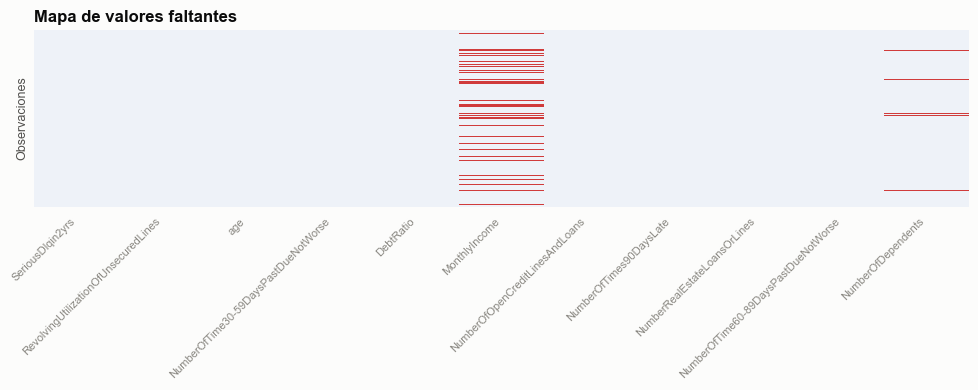
\includegraphics[width=0.85\textwidth]{fig_faltantes.png}
\caption{Mapa de valores faltantes del dataset. Solo \texttt{MonthlyIncome} y \texttt{NumberOfDependents} presentan datos nulos.}
\label{fig:faltantes}
\end{figure}

\subsubsection{Análisis univariado}

La Figura~\ref{fig:histogramas} presenta los histogramas de las diez variables numéricas. Se observa una fuerte asimetría positiva (cola derecha) en la mayoría de las variables, especialmente \texttt{RevolvingUtilizationOfUnsecuredLines}, \texttt{DebtRatio} y \texttt{MonthlyIncome} (asimetría de Fisher $\approx$ 98, 95 y 127, respectivamente, con curtosis en exceso del orden de miles), cuyos histogramas concentran casi toda la masa cerca de cero con una cola larga de valores extremos. La variable \texttt{age} es la que más se aproxima a una distribución simétrica (asimetría $\approx$ 0.19, curtosis en exceso $\approx -0.50$), aunque sigue siendo un conteo discreto en años completos. Las tres variables de conteo de atrasos muestran casi toda su masa en cero y un pico aislado en los valores 96 y 98, un código de valor especial documentado en el dataset original que no representa un conteo real de atrasos (Sección~\ref{subsubsec:anomalias}). En conjunto, estos diagnósticos de forma —asimetría marcada, curtosis extrema y naturaleza discreta con pocos valores únicos en varias variables— descartan a la distribución normal como modelo razonable para cualquiera de las diez variables, lo que sustenta el uso de estadísticos y pruebas no paramétricas en el resto del análisis.

\begin{figure}[h]
\centering
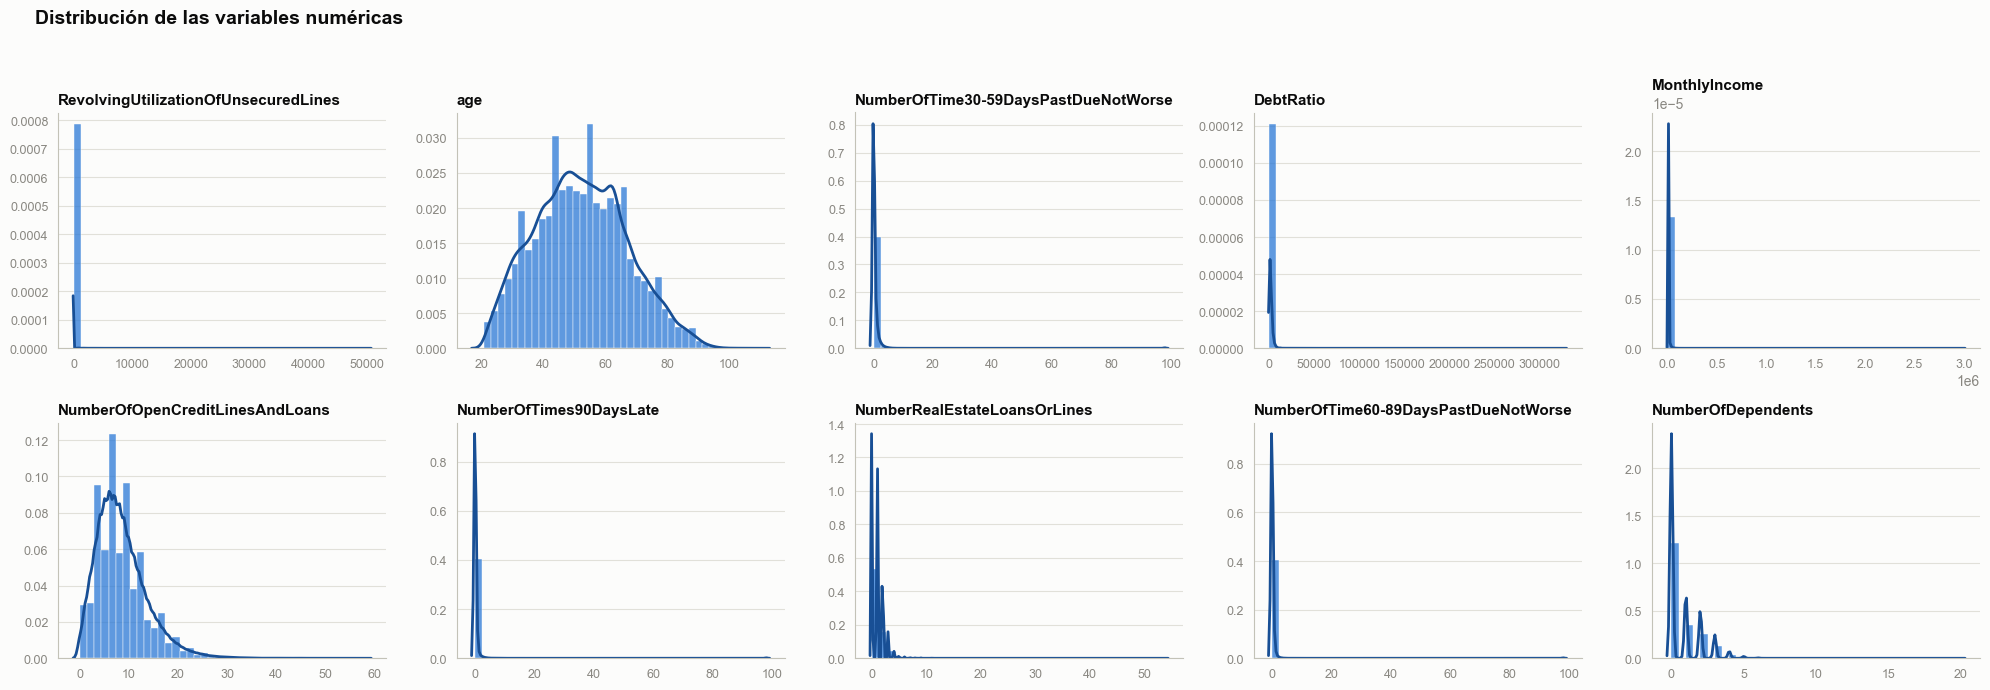
\includegraphics[width=\textwidth]{fig_histogramas.png}
\caption{Distribución (histograma + KDE) de las diez variables numéricas del dataset.}
\label{fig:histogramas}
\end{figure}

\subsubsection{Detección de valores atípicos}

La Figura~\ref{fig:boxplots} muestra los diagramas de caja de las diez variables numéricas. Se confirma la presencia de valores atípicos severos: las tres variables de conteo de atrasos presentan una desviación estándar muy superior a su media y un máximo de 98 asociado al código de valor especial ya mencionado; \texttt{RevolvingUtilizationOfUnsecuredLines}, \texttt{DebtRatio} y \texttt{MonthlyIncome} muestran máximos extremadamente alejados de su mediana, sugiriendo errores de captura o casos atípicos genuinos que deberán tratarse antes del modelamiento; y \texttt{age} presenta un valor mínimo de 0 años, un error de captura corregido en la etapa \textit{Transform} del ETL.

\begin{figure}[h]
\centering
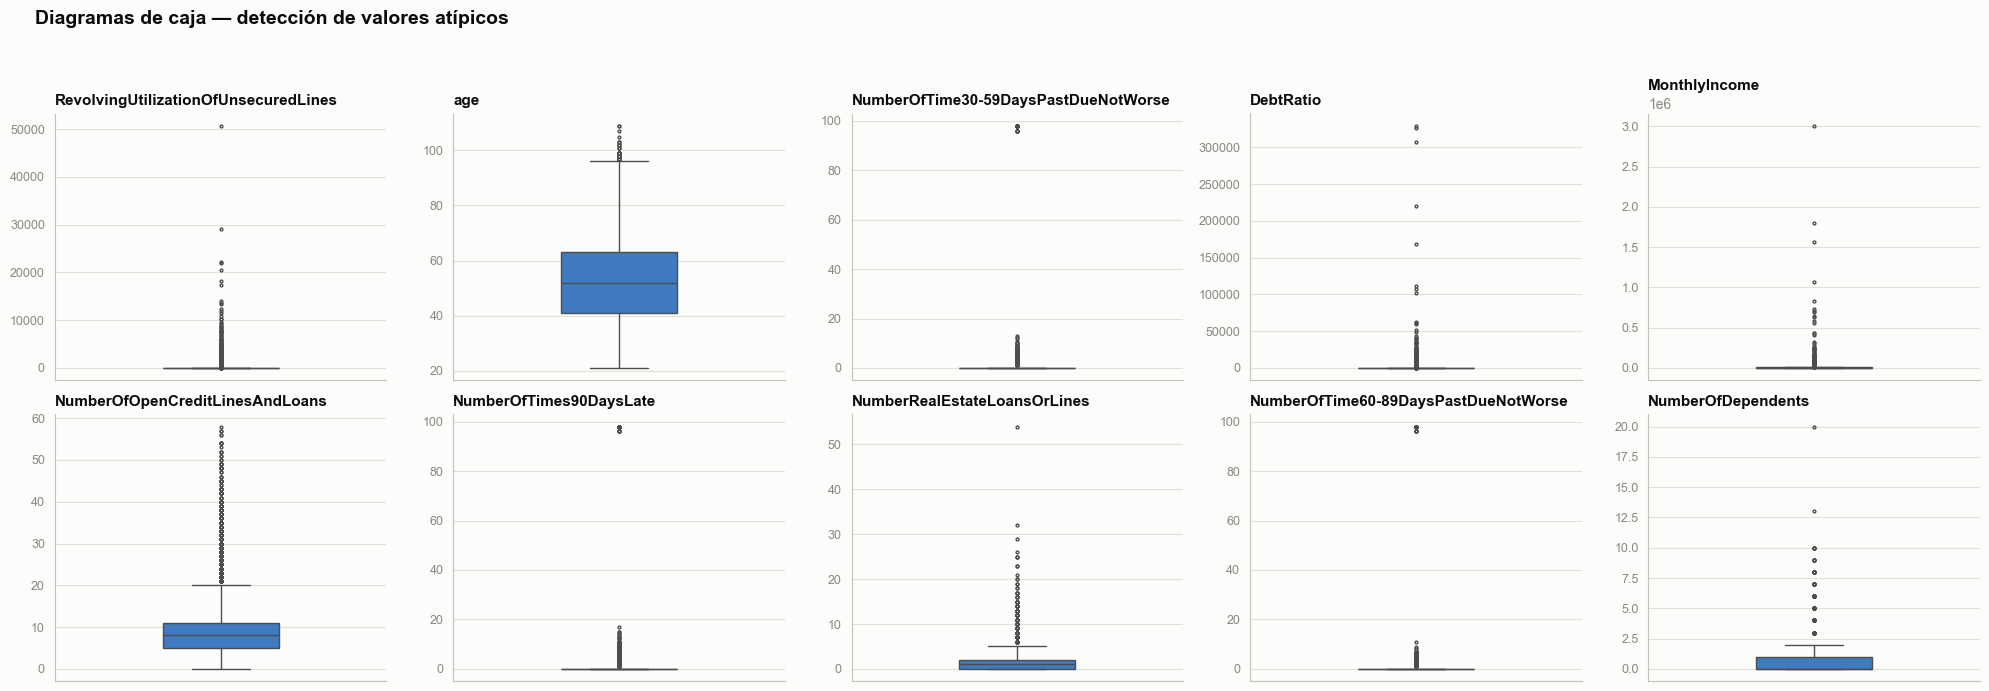
\includegraphics[width=\textwidth]{fig_boxplots.png}
\caption{Diagramas de caja de las diez variables numéricas, usados para la detección visual de valores atípicos.}
\label{fig:boxplots}
\end{figure}

\subsubsection{Tratamiento de anomalías: código especial de mora (96/98) y anomalía en \texttt{DebtRatio}}\label{subsubsec:anomalias}

Antes de calcular cualquier estadístico bivariado, prueba de hipótesis o correlación, se documentaron y trataron provisionalmente dos anomalías detectadas en las secciones anteriores.

\textbf{Código de valor especial en las variables de mora.} Las tres variables de conteo de atrasos (\texttt{NumberOfTime30-59DaysPastDueNotWorse}, \texttt{NumberOfTime60-89DaysPastDueNotWorse}, \texttt{NumberOfTimes90DaysLate}) presentan un pico aislado en los valores 96 y 98, muy alejado del resto de la distribución. Se identificaron 269 filas (0.179\%) con al menos una de estas variables en \{96, 98\}. Para evitar que este código contamine las medianas, las pruebas de hipótesis y la matriz de correlación de las secciones siguientes, dichos valores se reemplazaron temporalmente por \texttt{NaN} (excluidos de forma \textit{pairwise}, no \textit{listwise}) y se registró un indicador \texttt{flag\_codigo\_especial\_mora}. Este tratamiento es exclusivamente exploratorio: la decisión definitiva para el modelamiento (usar el indicador como variable de entrada, imputar por mediana documentando la bandera, o dejar el código sin tratar si se usan modelos de árboles) queda para la siguiente etapa del proyecto.

\textbf{Anomalía en \texttt{DebtRatio}.} La variable \texttt{DebtRatio} alcanza un máximo de 329{,}664, un valor sin interpretación financiera plausible para una razón deuda/ingreso, y supera 1 en el 23\% de los registros. Cruzando esta variable con el indicador \texttt{ingreso\_no\_reportado} (Sección~\ref{subsec:etl}) se explica el fenómeno: entre las 29{,}731 filas donde \texttt{MonthlyIncome} venía originalmente en blanco, el 93.85\% tiene \texttt{DebtRatio} > 1 (mediana $\approx$ 1{,}159), mientras que entre las 120{,}268 filas con ingreso reportado, solo el 6.01\% supera 1 (mediana $\approx$ 0.30, un valor razonable para una razón deuda/ingreso). Esto indica que, cuando el ingreso no estaba disponible, la columna \texttt{DebtRatio} contiene con alta probabilidad el pago de deuda absoluto (en dólares) y no una razón; la imputación de \texttt{MonthlyIncome} por mediana no corrige este problema, ya que no recalcula \texttt{DebtRatio} con el ingreso imputado. Al igual que con el código especial de mora, este EDA documenta el fenómeno sin corregirlo, dejando \texttt{ingreso\_no\_reportado} disponible como variable de segmentación o interacción para la fase de modelamiento.

\subsubsection{Variable objetivo}

La Figura~\ref{fig:balance} presenta la distribución de la variable objetivo \texttt{SeriousDlqin2yrs}. Se observa un desbalance de clases marcado: 93.32\% de los clientes (139{,}973) no presentó morosidad grave, frente a solo 6.68\% (10{,}026) que sí la presentó. Este desbalance es consistente con la naturaleza del problema —los eventos de incumplimiento grave son, por definición, poco frecuentes— y debe considerarse explícitamente en el modelamiento posterior (por ejemplo, mediante remuestreo, ponderación de clases o métricas distintas a la exactitud, como AUC o recall).

\begin{figure}[h]
\centering
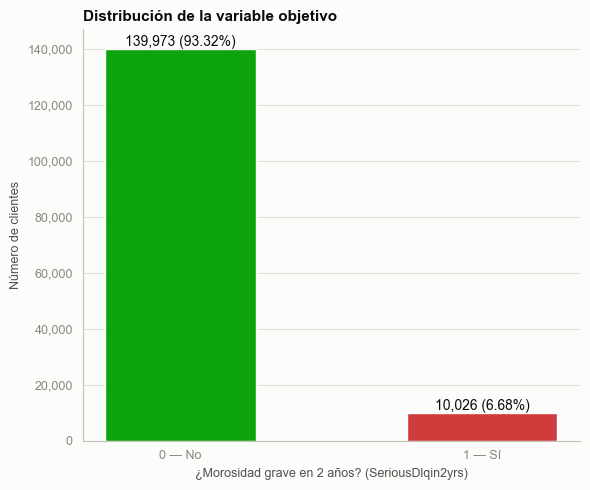
\includegraphics[width=0.5\textwidth]{fig_balance_clases.png}
\caption{Distribución de la variable objetivo \texttt{SeriousDlqin2yrs}, evidenciando el desbalance hacia la clase 0 (sin morosidad grave).}
\label{fig:balance}
\end{figure}

\subsubsection{Análisis bivariado y comparación formal de grupos}\label{subsubsec:bivariado}

Para el análisis bivariado se seleccionaron ocho variables numéricas: las cinco variables de interés de negocio originales (\texttt{age}, \texttt{RevolvingUtilizationOfUnsecuredLines}, \texttt{DebtRatio}, \texttt{MonthlyIncome}, \texttt{NumberOfOpenCreditLinesAndLoans}) más las tres variables de conteo de atrasos, una vez tratado el código especial 96/98 como se describió en la Sección~\ref{subsubsec:anomalias}. Se excluyeron únicamente \texttt{NumberRealEstateLoansOrLines} y \texttt{NumberOfDependents}, por ser de menor interés de negocio directo, no por problemas de calidad de datos. La Figura~\ref{fig:bivariado} compara cada variable frente a la variable objetivo mediante diagramas de caja, marcando la media de cada grupo. La Tabla~\ref{tab:bivariado} resume la mediana de cada variable por grupo; para las tres variables de mora, la mediana es 0 en ambos grupos (la mayoría de los clientes no registra atrasos), por lo que la diferencia porcentual no es informativa ahí, aunque sí exista una diferencia real más arriba en la distribución. La variable con mayor diferencia relativa de medianas es \texttt{RevolvingUtilizationOfUnsecuredLines} (mediana de 0.13 en clientes sin morosidad grave frente a 0.84 en clientes con morosidad grave, +529.4\%).

\begin{figure}[h]
\centering
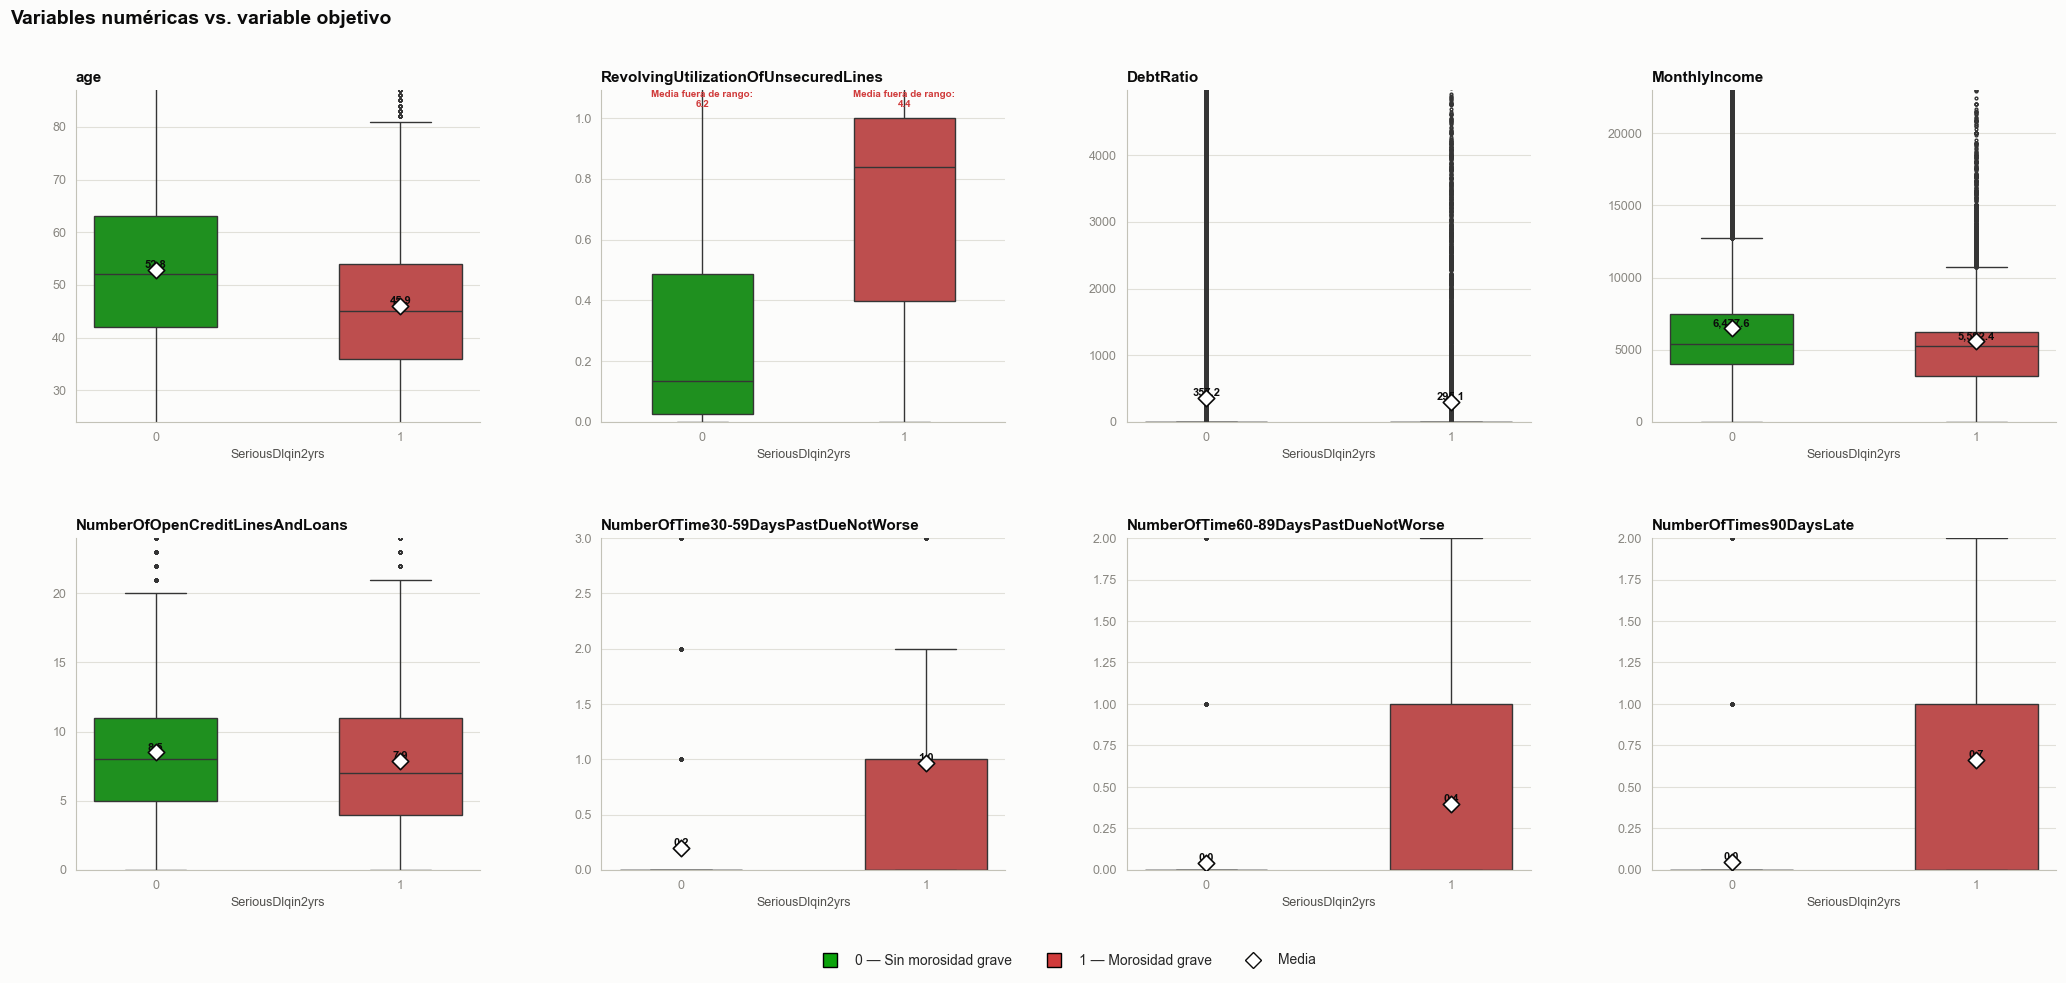
\includegraphics[width=\textwidth]{fig_bivariado_fixed.png}
\caption{Diagramas de caja de las ocho variables numéricas seleccionadas frente a la variable objetivo \texttt{SeriousDlqin2yrs} (eje y recortado entre percentiles 1 y 99 para facilitar la comparación visual; los valores atípicos permanecen en los datos; el rombo blanco marca la media de cada grupo).}
\label{fig:bivariado}
\end{figure}

\begin{table}[h]
\centering
\caption{Mediana de cada variable según la variable objetivo \texttt{SeriousDlqin2yrs}.}\label{tab:bivariado}
\begin{tabular}{@{}lccc@{}}
\toprule
Variable & Mediana (0) & Mediana (1) & Diferencia (\%) \\
\midrule
age & 52.00 & 45.00 & $-13.5$ \\
RevolvingUtilizationOfUnsecuredLines & 0.133 & 0.839 & $+529.4$ \\
DebtRatio & 0.363 & 0.428 & $+18.1$ \\
MonthlyIncome & 5400.0 & 5240.0 & $-3.0$ \\
NumberOfOpenCreditLinesAndLoans & 8.00 & 7.00 & $-12.5$ \\
NumberOfTime30-59DaysPastDueNotWorse & 0.00 & 0.00 & — \\
NumberOfTime60-89DaysPastDueNotWorse & 0.00 & 0.00 & — \\
NumberOfTimes90DaysLate & 0.00 & 0.00 & — \\
\botrule
\end{tabular}
\end{table}

Dado el tamaño muestral (N $\approx$ 150{,}000, con subgrupos de decenas de miles de observaciones), cualquier prueba formal de bondad de ajuste a la normalidad (Kolmogorov--Smirnov, Shapiro--Wilk, Lilliefors) o de homogeneidad de varianzas (Levene) sufre de exceso de potencia estadística: al crecer $N$, la potencia de la prueba tiende a 1 y termina rechazando la hipótesis nula ante desviaciones triviales sin relevancia práctica. Por esta razón, no se ejecutaron dichas pruebas formales; la decisión de usar métodos no paramétricos se apoya en su lugar en los diagnósticos descriptivos de forma ya presentados (asimetría, curtosis y naturaleza discreta, Sección~\ref{subsubsec:anomalias} y Tabla~\ref{tab:descriptivos}), que descartan la normalidad en las ocho variables y en ambos grupos.

Con base en esos diagnósticos, se aplicó la prueba de Mann--Whitney U de forma uniforme a las ocho variables, interpretada como una prueba de dominancia estocástica y no de un simple contraste de medianas, dado que las formas de las distribuciones difieren entre grupos. Como el p-valor por sí solo pierde utilidad a este tamaño muestral (prácticamente cualquier diferencia real resulta significativa), se reportan además dos medidas de tamaño de efecto: la $r$ de Rosenthal ($r = |Z|/\sqrt{N}$, con la corrección estándar de Hogg--Craig por empates) y el AUC univariado ($= P(\text{valor en grupo 1} > \text{valor en grupo 0})$), que mide qué tan bien discrimina cada variable por sí sola. La Tabla~\ref{tab:mannwhitney} resume los resultados.

\begin{table}[h]
\centering
\caption{Resultados de la prueba de Mann--Whitney U (dos colas) entre clientes con y sin morosidad grave, con tamaño de efecto $r$ de Rosenthal (corregido por empates) y AUC univariado. Variables ordenadas de mayor a menor tamaño de efecto.}\label{tab:mannwhitney}
\small
\begin{tabular}{@{}lcccc@{}}
\toprule
Variable & $p$-valor & $r$ de Rosenthal & Tamaño de efecto & AUC \\
\midrule
NumberOfTimes90DaysLate & $<0.001$ & 0.335 & mediano & 0.653 \\
NumberOfTime60-89DaysPastDueNotWorse & $<0.001$ & 0.268 & pequeño & 0.617 \\
NumberOfTime30-59DaysPastDueNotWorse & $<0.001$ & 0.251 & pequeño & 0.686 \\
RevolvingUtilizationOfUnsecuredLines & $<0.001$ & 0.240 & pequeño & 0.778 \\
age & $<0.001$ & 0.117 & pequeño & 0.365 \\
MonthlyIncome & $3.48\times10^{-126}$ & 0.062 & trivial & 0.429 \\
NumberOfOpenCreditLinesAndLoans & $1.68\times10^{-50}$ & 0.039 & trivial & 0.455 \\
DebtRatio & $1.50\times10^{-15}$ & 0.021 & trivial & 0.524 \\
\botrule
\end{tabular}
\end{table}

Las ocho variables resultan estadísticamente significativas ($p < 0.05$ en todos los casos), lo cual es esperable a este tamaño de muestra y confirma que el $p$-valor no es, por sí solo, un criterio útil aquí. Ordenando por tamaño de efecto, \texttt{NumberOfTimes90DaysLate} tiene la mayor capacidad discriminativa (r $\approx$ 0.34, AUC $\approx$ 0.65), seguida de las otras dos variables de mora y de \texttt{RevolvingUtilizationOfUnsecuredLines} (r $\approx$ 0.24, con el AUC univariado más alto de las ocho, $\approx$ 0.78). \texttt{age} tiene efecto pequeño (r $\approx$ 0.12) con AUC por debajo de 0.5, lo que indica que los clientes con morosidad grave tienden a ser más jóvenes, no mayores. En el otro extremo, \texttt{DebtRatio}, \texttt{MonthlyIncome} y \texttt{NumberOfOpenCreditLinesAndLoans} tienen tamaño de efecto trivial (r < 0.10, AUC cercano a 0.5): son estadísticamente significativas por el tamaño de muestra, no porque discriminen de forma relevante entre clientes con y sin morosidad grave.

\subsubsection{Correlación entre variables predictoras}

Dado que ninguna variable se comporta como normal continua, se utilizó el coeficiente de correlación de Spearman entre las variables predictoras numéricas, con el fin de detectar posibles relaciones fuertes o redundancias (multicolinealidad) antes de construir un modelo (Figura~\ref{fig:correlacion}). Las dos relaciones más fuertes identificadas fueron \texttt{NumberOfOpenCreditLinesAndLoans} con \texttt{NumberRealEstateLoansOrLines} ($\rho = 0.47$, correlación positiva moderada) y \texttt{DebtRatio} con \texttt{NumberRealEstateLoansOrLines} ($\rho = 0.40$, correlación positiva moderada), mostradas en la Figura~\ref{fig:relaciones}. En ambos casos la magnitud de la correlación no sugiere redundancia relevante entre las variables involucradas.

\begin{figure}[h]
\centering
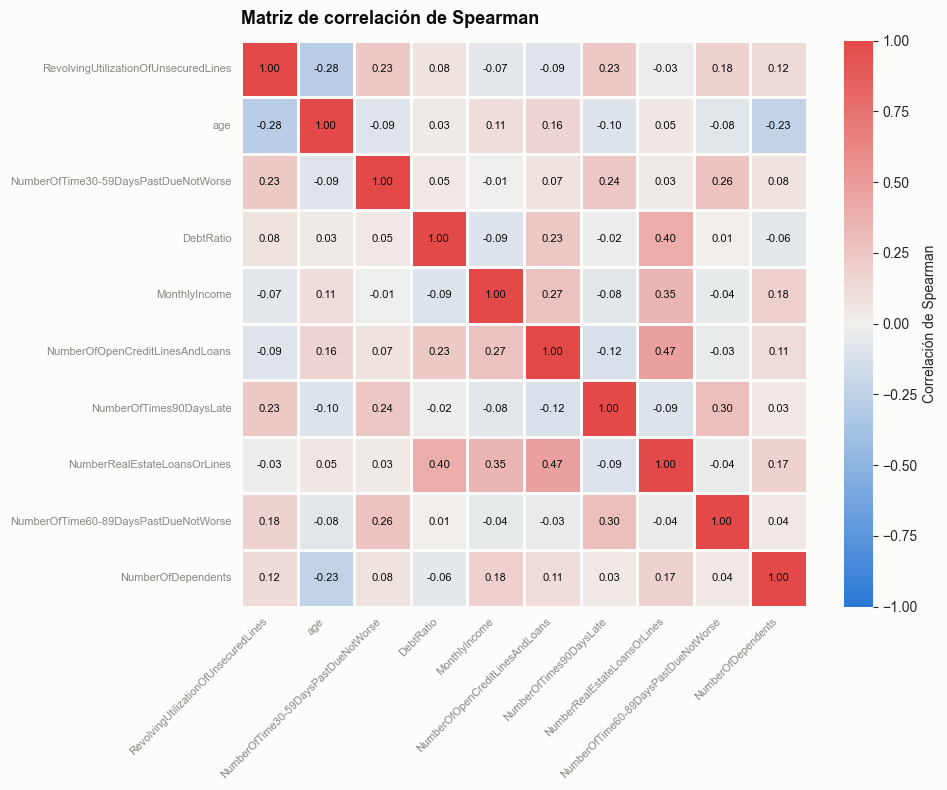
\includegraphics[width=0.7\textwidth]{fig_correlacion.png}
\caption{Matriz de correlación de Spearman entre las variables predictoras numéricas.}
\label{fig:correlacion}
\end{figure}

\begin{figure}[h]
\centering
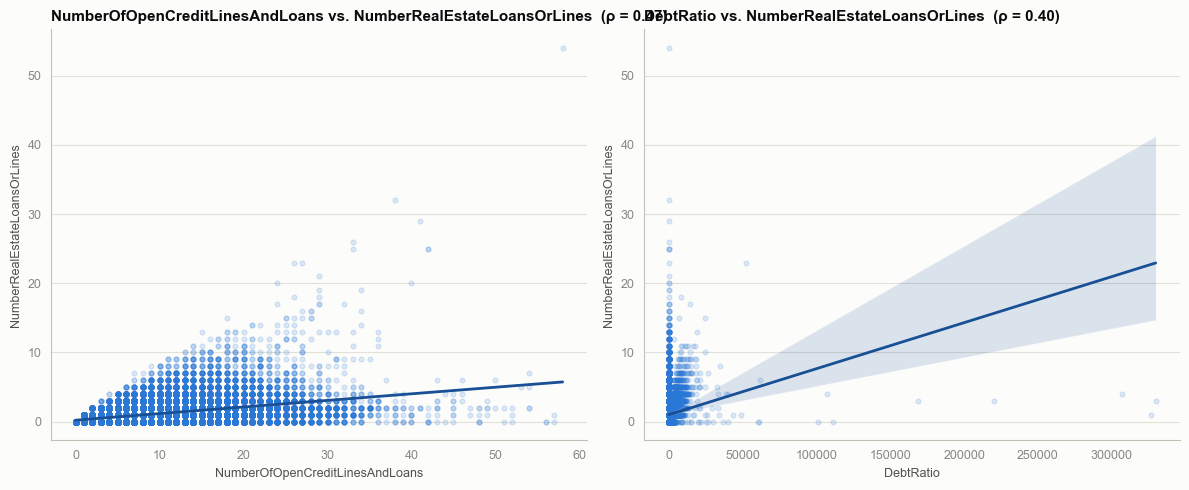
\includegraphics[width=\textwidth]{fig_relaciones.png}
\caption{Diagramas de dispersión de las dos relaciones bivariadas más fuertes según la correlación de Spearman: \texttt{NumberOfOpenCreditLinesAndLoans} vs. \texttt{NumberRealEstateLoansOrLines} ($\rho = 0.47$) y \texttt{DebtRatio} vs. \texttt{NumberRealEstateLoansOrLines} ($\rho = 0.40$).}
\label{fig:relaciones}
\end{figure}

\subsubsection{Conclusiones del EDA y decisiones de preprocesamiento}

Como consecuencia directa de los hallazgos del EDA, se tomaron las siguientes decisiones de preprocesamiento en la etapa \textit{Transform} del ETL: (i) imputación por mediana de \texttt{MonthlyIncome} y \texttt{NumberOfDependents}, dada su asimetría y el volumen de valores faltantes, conservando el indicador \texttt{ingreso\_no\_reportado} para uso posterior; (ii) eliminación del registro con \texttt{age} = 0, por tratarse de un error de captura evidente; y (iii) el código de valor especial (96/98) de las variables de mora y la anomalía de \texttt{DebtRatio} se documentaron y se trataron únicamente de forma provisional para los cálculos de este EDA (indicadores \texttt{flag\_codigo\_especial\_mora} e \texttt{ingreso\_no\_reportado}), quedando su tratamiento definitivo (dummy, imputación documentada, segmentación o transformación robusta como \textit{winsorización} o logarítmica) pendiente para la etapa de modelamiento. Adicionalmente, el marcado desbalance de clases de la variable objetivo (93.32\% vs. 6.68\%) deberá abordarse mediante estrategias como remuestreo (por ejemplo, ADASYN~\cite{chia2025adasyn}), ponderación de clases o el uso de métricas de evaluación distintas a la exactitud (AUC, recall, F1-score), dado que un modelo entrenado sin considerar este desbalance tendería a favorecer trivialmente a la clase mayoritaria~\cite{ichim2025credit}.

\section{Conclusiones}\label{sec:conclusiones}

Esta primera fase del proyecto completó satisfactoriamente el proceso de ETL y un Análisis Exploratorio de Datos exhaustivo sobre el conjunto \textit{Give Me Some Credit}, dejando un dataset limpio (149{,}999 filas, sin valores faltantes) y una comprensión detallada de su estructura. Los hallazgos más relevantes —el fuerte desbalance de clases, la asimetría positiva de las variables financieras, el código de valor especial 96/98 en las variables de mora, la anomalía de \texttt{DebtRatio} explicada por el ingreso no reportado, y la jerarquía de poder discriminativo revelada por Mann--Whitney U (encabezada por \texttt{NumberOfTimes90DaysLate} y \texttt{RevolvingUtilizationOfUnsecuredLines}, con \texttt{DebtRatio}, \texttt{MonthlyIncome} y \texttt{NumberOfOpenCreditLinesAndLoans} de efecto trivial pese a su significancia estadística)— se traducen directamente en decisiones concretas de preprocesamiento que quedan documentadas como insumo para la siguiente etapa.

Como limitación de esta fase, el tratamiento del código de valor especial y de la anomalía de \texttt{DebtRatio} se documentó pero solo se aplicó de forma provisional para los cálculos del EDA, por lo que el dataset actual no está listo para el modelamiento sin ese paso adicional. Como trabajo futuro, las siguientes etapas del proyecto abordarán dicho tratamiento definitivo, la selección y el entrenamiento de modelos de clasificación (incluyendo estrategias para el desbalance de clases), y la evaluación comparativa de su desempeño frente a los modelos vistos en el curso.

\backmatter

\section*{Declaraciones}

\begin{itemize}
\item \textbf{Disponibilidad de datos:} el conjunto \textit{Give Me Some Credit} es público y puede descargarse desde Kaggle (\url{https://www.kaggle.com/c/GiveMeSomeCredit}).
\item \textbf{Disponibilidad de código:} el código fuente en Python y los cuadernos de Jupyter para la reproducción del ETL y el EDA están disponibles en el repositorio del proyecto: \url{https://github.com/valeriaflorezs/GiveMeSomeCredit}.
\item \textbf{Contribución de los autores:} V. Flórez y K. Barrera diseñaron la metodología, ejecutaron el procesamiento de datos, realizaron el análisis exploratorio y redactaron el manuscrito. Ambas autoras revisaron y aprobaron la versión final.
\item \textbf{Conflicto de intereses:} las autoras declaran no tener conflictos de interés.
\end{itemize}

\bibliography{sn-bibliography}

\end{document}
